%%%%%%%%%%%%%%%%%%%% author.tex 
%%%%%%%%%%%%%%%%%%%%%%%%%%%%%%%%%%%
%
% sample root file for your "contribution" to a proceedings volume
%
% Use this file as a template for your own input.
%
%%%%%%%%%%%%%%%% Springer 
%%%%%%%%%%%%%%%%%%%%%%%%%%%%%%%%%%


\documentclass{svproc}
%
% RECOMMENDED 
%%%%%%%%%%%%%%%%%%%%%%%%%%%%%%%%%%%%%%%%%%%%%%%%
%%%
%
\usepackage{graphicx}
\usepackage{marvosym}

%\pdfmapfile{+txfonts.map}

%\usepackage[utf8]{inputenc}
%\usepackage[english, russian]{babel} % ������� � ���������� ��������

% to typeset URLs, URIs, and DOIs
\usepackage{url}
\usepackage{hyperref}
\def\UrlFont{\rmfamily}

\def\orcidID#1{\unskip$^{[#1]}$}
\def\letter{$^{\textrm{(\Letter)}}$}

\begin{document}
\mainmatter              % start of a contribution
%
\title{Combining of local and global search in the parallel nested optimization scheme 
\thanks{This study was supported by the Russian Science Foundation, project No.\,16-11-10150.}
}
%
\titlerunning{Combining of local and global search}  % abbreviated title (for running head)
%                                     also used for the TOC unless
%                                     \toctitle is used
%
\author{Konstantin Barkalov\letter\orcidID{0000-0001-5273-2471} \and Ilya 
Lebedev\orcidID{0000-0002-8736-0652} \and Maria Kocheganova \orcidID{0000-0002-4722-6299} 
\and Victor Gergel \orcidID{0000-0002-4013-2329}}
%
\authorrunning{Konstantin Barkalov et al.} % abbreviated author list (for running head)
%
%%%% list of authors for the TOC (use if author list has to be modified)
\tocauthor{Konstantin Barkalov and Ilya Lebedev, and Maria Kocheganova}
%
\institute{Lobachevsky State University of Nizhni Novgorod, Russia  \\
	\email{konstantin.barkalov@itmm.unn.ru}
}
	
\maketitle              % typeset the title of the contribution

\begin{abstract}

In the present paper, the global optimization problems and the numerical methods of solving these 
ones are considered. 
Regarding the character of the dependence of the objective function on its parameters, an assumption 
is made that it is multiextremal with respect to selected variables only, and the dependence on the rest 
ones has a local character. 
The problems of this type may arise in the identification of the unknown parameters of the 
mathematical models on the base of the results of experiments. 
A parallel computational scheme, which accounts for this feature has been proposed.
The novel scheme is based on the idea of the nested (recursive) optimization when at the upper 
recursion level the optimization with respect to the globally-meaning variables is performed (using 
the global optimization method), and at the lower one the local optimization problems are solved (using 
the local method). The generated local subproblems will not affect each other, and solving of these 
ones can be performed in parallel. The numerical experiments have been conducted on several 
hundred test problems confirming the efficiency of the proposed scheme of parallel computations.


\keywords{Global optimization $\cdot$ Local optimization $\cdot$ Recursive optimization scheme 
$\cdot$ Parallel algorithms}
\end{abstract}

\section{Introduction}

The global optimization problems arise often in various fields of modern science and technology. For 
example, the problems of finding the configurations of various chemical compounds corresponding to 
the minimum interaction energy are relevant \cite{Posypkin2014}. In particular,  such problems arise 
in the development of new medical drugs \cite{Sulimov}. 
Another example is the problem of finding optimal control parameters for complex processes \cite{Kalyulin2017,Modorskii2016}.
The global optimization problems arise in many other applications as well (see the review \cite{Pinter2006}). 

The application of the global optimization methods for the identification of the parameters of the 
mathematical models based on the data of experiments became a classical one. In the problems of this 
type, it is required to carry out a search for the values of the unknown parameters of the model, at 
which the results of computations according to the model are close to the results obtained 
experimentally.

The number of parameters, which are required to be identified in such a way may be tens and hundreds 
in complex mathematical models \cite{Akhmadullina2017,Nurislamova2016}. In the problems of 
such dimensionality, the regular methods of search for the global solutions cannot be applied because 
of extremely large computational costs for covering the search domain by the trial points. This 
remains to be true even in the case of the use of efficient algorithms (for example, 
\cite{Evtushenko2009,Jones2009,Paulavicius2011}) constructing essentially nonuniform coverages. 

However, in the problems of the model identification, the parameters, which will affect the result 
mostly can be selected often. The number of such parameters is small as a rule. The rest parameters 
either cause an insufficient effect (in this case, the multiextremality can be neglected) or the 
dependence on the second group of parameters have a local character.

So far, the development of the parallel algorithms for the minimization of the essentially 
multidimensional functions (hundreds of variables), which account for different character of 
dependence of the objective function on different groups of parameters is relevant. Namely, the 
objective function is assumed to be multiextremal with respect to a part of variables only. The rest 
variables have a local effect, i.e. the objective function is unimodal with respect to these ones. 
In this case, the solving of the problem can be organized according to the nested (recursive) 
optimization scheme. The solving of the multiextremal subproblem, for which the use of complex 
global search algorithms is required, will be performed at the upper level of recursion.
The unimodal subproblems (each corresponding to a fixed set of values of the first part of 
parameters) will be solved at the lower level. For solving these subproblems, the efficient 
methods of local optimization, linear programming, or linear algebra can be applied (subject to the 
character of the local subproblems).

The paper text describing the results of the present study is organized as follows. 
In Section 2, the description of the nested optimization scheme taking into account different properties 
of the objective function at different nesting level is given. Particular example of a problem of this 
class is presented. A general scheme of organization of the parallel computations is described. 
Section 3 is devoted to the description of the parallel global search algorithm using the space-filling 
curves. The computational scheme of the parallel algorithm is presented, its main properties are 
described.
In Section 4, the methods of solving the local subproblems within the framework of the nested 
optimization scheme are discussed. A brief description of the properties of the local extremum search 
problems and known methods of solving these ones is given. 
Section 5 contains the results of numerical experiment. Here, the evaluation of the scalability of the 
proposed parallel computation scheme in solving a series of test problems is performed.  
Section 6 concludes the paper.


\section{Nested optimization scheme}

Let us consider an optimization problem of the type
\begin{eqnarray}\label{main_problem}
& f(x^\ast,y^\ast)=\min{\left\{f(x,y):x\in S, y\in D\right\}}, \nonumber \\
& S=\left\{x\in R^M: a_i\leq x_i \leq b_i, 1\leq i \leq M\right\}, \\
& D=\left\{y\in R^N: c_i\leq y_i \leq d_i, 1\leq i \leq N\right\}. \nonumber
\end{eqnarray}

Let us assume that at any fixed set of the values $\overline{x}$ the function $f(\overline{x},y)$ is a 
multiextremal one and satisfies Lipschitz condition
\[
\left|f(\overline{x},y')-f(\overline{x},y'')\right|\leq L\left\|y'-y''\right\|,\; y',y'' \in D,\; 0<L<\infty,
\]
with the constant $L$ unknown a priori.
At the same time, at any fixed set of values $\overline{y}$ the function $f(x,\overline{y})$ is a 
unimodal one, i.e. the function $f(x,\overline{y})$ has a single minimum point $x^*$ (depending, in 
general, on $\overline{y}$). 

Accounting for such a peculiarity of the considered problem class can reduce essentially the computational costs 
of the optimum search. Indeed, according to known nested optimization scheme 
\cite{Carr}, the solving of the initial problem can be reduced to the problem of finding the global 
minimum of the function $\varphi(y)$
\begin{equation}\label{global_problem}
\varphi(y^*) = \min_{y\in D}  \varphi (y),
\end{equation}
where 
\begin{equation}\label{local_problem}
\varphi(y) = \min_{x\in S} f(x,y).
\end{equation}
According to (\ref{global_problem}), the computing of a single value of the function $\varphi (y)$ 
(let us call this process a search trial) implies the solving of a unimodal problem (\ref{local_problem}), 
which can be performed by one of the local search methods. The efficiency and sophistication of the 
local optimization methods allow solving the subproblems (\ref{local_problem}) with the precision 
exceeding the one of the global optimization methods essentially. Correspondingly, the problem 
(\ref{global_problem}) can be considered as a global optimization problem, in which the objective 
function value can be computed with high precision but this operation is time-consuming. 

The following approximation problem can be considered as a particular example of a problem, in 
which different character of dependence on different groups of parameters takes place. 
Let us assume $m$ values $u_j = u(t_j), 1 \leq j \leq m, $ of the function $u(t)$ to have been obtained 
in the experiment and the analytical expression for $u(t)$ is known to take the form 
\begin{equation}\label{ex_func}
u(t) = u(t,\omega,c)=\sum^{n}_{i=0}\left[c_{2i+1}\sin(\omega_it) + c_{2i+2}\cos(\omega_it)\right].	
\end{equation}
In this expression, $c=\left(c_1,\ldots,c_{2n+2}\right)$, 
$\omega=\left(\omega_0,\omega_1,\ldots,\omega_n\right)$ are the unknown parameters defining 
particular function $u(t)$.

Let us introduce a measure of the deviation of the function $u(t,\omega,c)$ from the experiential data as a 
sum of squares 
\[
\Delta(\omega,c)= \sum^{m}_{j=1}\left[u_j-u(t_j,\omega,c)\right]^2. 
\]
Now, following the idea of least squares fitting, it is possible to present the approximation problem as 
the problem of minimizing the objective function
\begin{equation}\label{ex_prob}
\Delta(\omega^*,c^*) = \min_{\omega,c} \Delta(\omega,c).	
\end{equation}
The solution $(\omega^*,c^*)$ of this problem will define the best approximation.

The problem (\ref{ex_prob}) can be written in a recursive form 
\begin{equation}\label{outer_prob}
\varphi(\omega^*) = \min_\omega \varphi(\omega)
\end{equation}
\begin{equation}\label{inner_prob}
\varphi(\omega) = \min_c \Delta(\omega,c).
\end{equation}
The nested subproblem (\ref{inner_prob}) is a classical linear least squares problem, and its solution 
can be obtained by solving a system of linear algebraic equations regarding the unknown $c$, which 
can be done e.g. by Gaussian elimination. At the same time, the external problem (\ref{outer_prob}) 
will be, in general, a multiextremal one, and its solving will require considerable 
computational resources.

So far, to solve the problem (\ref{main_problem}) in the nested scheme (\ref{global_problem}), 
(\ref{local_problem}) one can apply parallel global search algorithm for solving the external 
subproblems (\ref{global_problem}). At that, a set of independent subproblems (\ref{local_problem}) 
will be generated at every iteration of the algorithm, the solving of which can be performed in parallel 
using the local methods.
A general scheme of the organization of the computations using several processors is presented in 
Fig.~\ref{MPI_tree}. 

\begin{figure}
\center{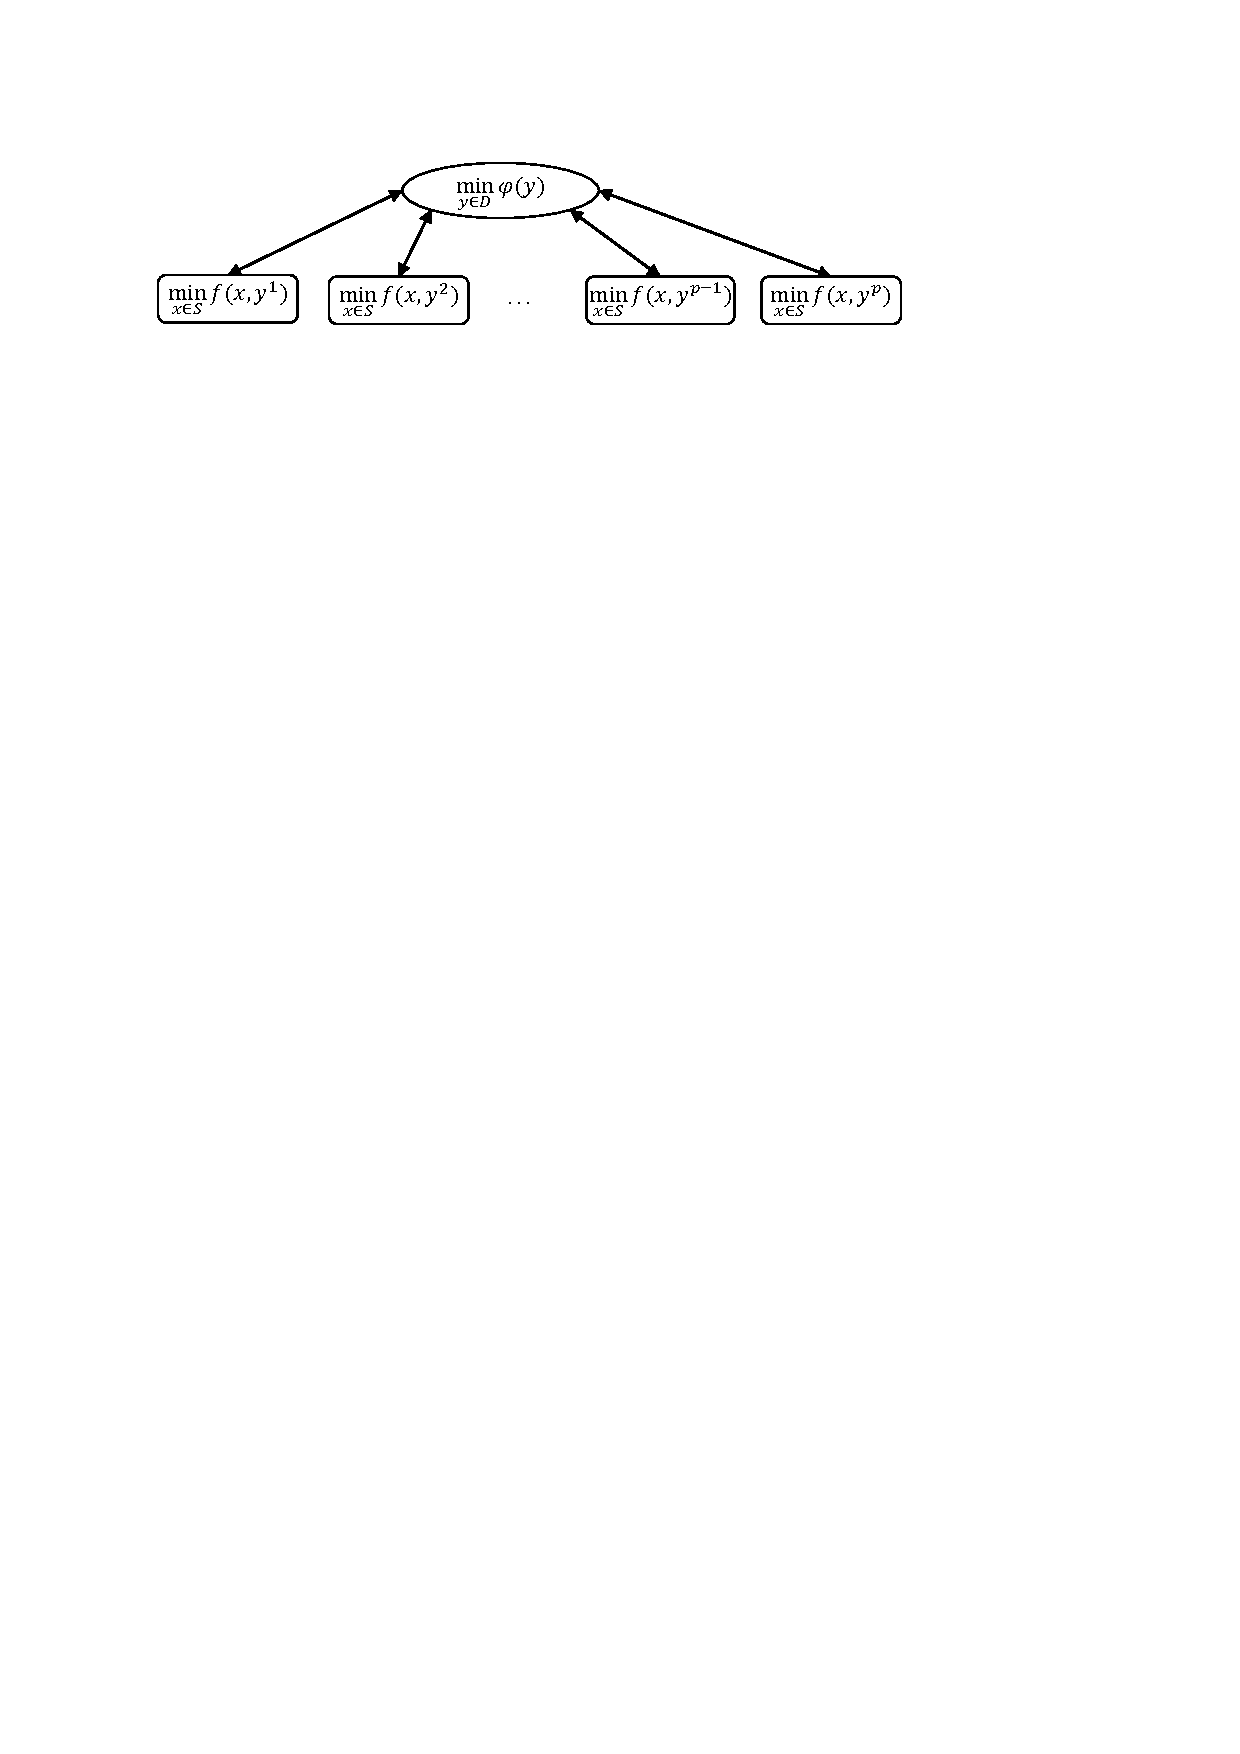
\includegraphics[width=1.0\linewidth]{MPI_Tree.pdf}}
\caption{A tree of subproblems in the parallel nested optimization scheme}
\label{MPI_tree}
\end{figure}

The processes of the parallel program will form a tree. 
The root process will solve the problem (\ref{global_problem}) and distribute the subproblems 
(\ref{local_problem}) among the child processes. Each subproblem is solved by a separate process, 
the data exchange between the processes can be organized using MPI. The data transmission between 
the processes will be minimal: it is required to send the coordinates of points $y^1, ..., y^p$ from the 
root to the child processes and to receive back the found minimal values 
\[
\varphi(y^1) = \min_x f(x,y^1),\; ..., \; \varphi(y^p) = \min_x f(x,y^p).
\]

A detailed discussion of the algorithms used at different levels of the process tree is given in the next 
sections. 

\section{Parallel global search algorithm}

An efficient parallel global optimization algorithm intended for solving the problems of the kind 
(\ref{global_problem}) has been developed in Lobachevsky University of Nizhni Novgorod (UNN) 
\cite{Barkalov2018,globalizerSystem,Strongin2018}. 
The main idea of the parallelization consists in such of organization of computations that several trials 
are performed in parallel. This approach is featured by high efficiency (the part of the computational 
process is parallelized, in which the major amount of computations is performed) and generality (it is 
applicable for a wide class of algorithms).

In the developed global search algorithm, a novel method for the reduction of the dimensionality of 
the problems to be solved is applied. 
The reduction of the dimensionality is based on a fundamental fact, according to which an 
$N$-dimensional hyperparallelepiped $D$ and the interval $[0,1]$ of the real axis are the 
equal-power sets, and the interval $[0,1]$ can be mapped continuously into $D$ using the Peano 
curve $y(x)$, i.e. $D = \left\{y(x):0\leq x\leq 1\right\}$.

Utilizing this fact, one can reduce the solving of the problem of minimization of a multidimensional 
function $\varphi(y)$ to the minimization of a one-dimensional function $\varphi(y(x))$
\begin{equation}\label{1d_problem}
\varphi(y (x^*)) = \min \left\{ \varphi (y(x)) : x\in [0,1] \right\},
\end{equation}
where the function $\varphi(y(x))$ will satisfy a uniform H{\"o}lder condition
\[
\left|\varphi(y(x'))-\varphi(y(x''))\right|\leq H\left|x'-x''\right|^{1/N}
\]
with the H{\"o}lder constant $H$ linked to the Lipschitz constant $L$ by the relation
$ H=2 L \sqrt{N+3}$ and $y(x)$ is the Peano curve from $[0,1]$ onto $D$.

The algorithms for the numerical construction of the Peano curve approximations (called 
\textit{evolvents})
are given in \cite{Sergeyev2013,Strongin2000}. As an illustration, two evolvents are shown in 
Fig.~\ref{fig_evolvent}. Figure demonstrates that the precision of the evolvent is depend on the 
density level $m$ used in the construction.

\begin{figure}
\center
\begin{minipage}{0.48\linewidth}
\center{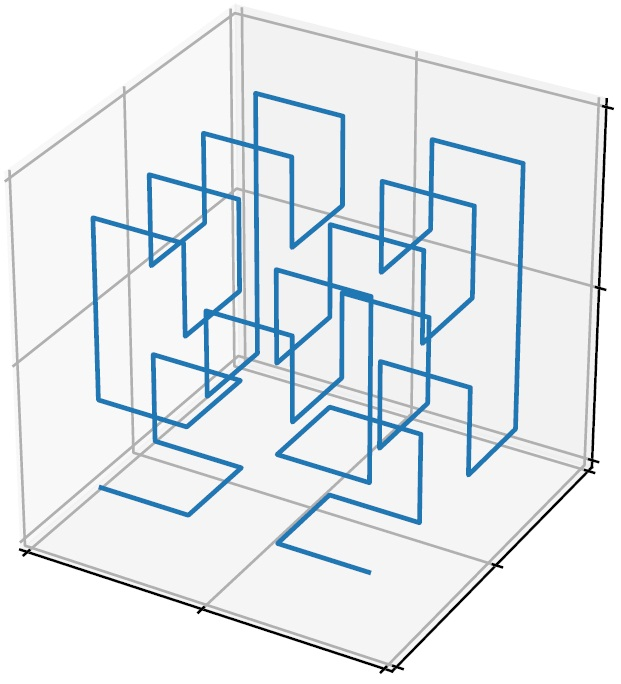
\includegraphics[width=1.0\linewidth]{fig1b.JPG} \\ (a)}
\end{minipage}
\begin{minipage}{0.48\linewidth}
\center{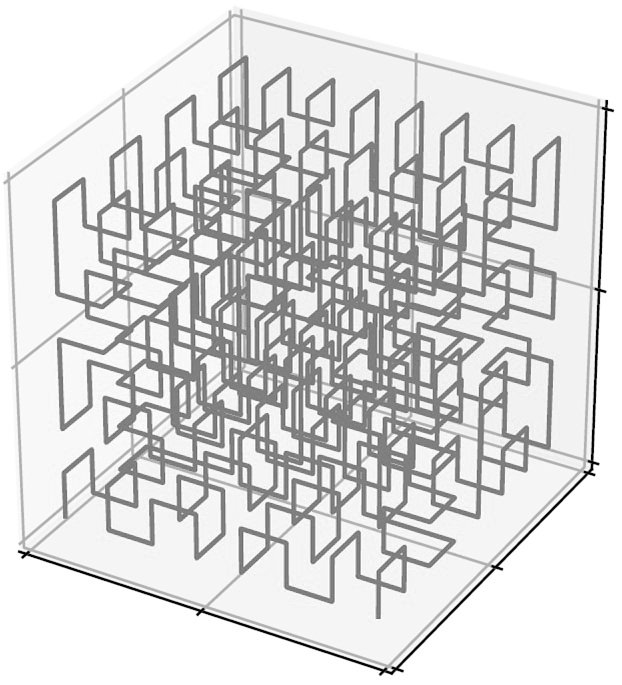
\includegraphics[width=1.0\linewidth]{fig1c.JPG} \\ (b)}
\end{minipage}
\caption{Evolvents in two dimensions with (a) $m=4$ and (b) $m=5$}
\label{fig_evolvent}
\end{figure}

It is worth noting that many well known global optimization algorithms are based implicitly on the 
idea of the dimensionality reduction and adaptation of the one-dimensional algorithms for solving the 
multidimensional problems \cite{Evtushenko2013,Sergeyev2006,Zilinskas2008}.

According to \cite{Strongin2018,Strongin2000}, the rules of the global search algorithm, in which 
$p$ trials are performed in parallel at every iteration, are as follows.
At the first iteration of the method, the trials are performed in parallel in two boundary points $x^1 = 
0, \; x^2 = 1$ as well as in $(p-2)$ arbitrary internal points of the interval $[0,1]$, i.e. 
$x^i\in(0,1),3\leq i \leq p$.

%English begin
Suppose $n\geq 1$  iterations of the method have been carried out, in which trials were performed at 
$k=k(n)$ points $x^i,1\leq i \leq k$. Then points $x^{k+1},\dots,x^{k+p}$  of search trials of the next 
iteration are determined according to the following rules.

Rule 1. Renumber the points $x^1,...,x^k$ of the preceding trials by the
lower indices in ascending order of coordinate values, i.e.
\[
0=x_1<x_2<\dots <x_{k-1} <x_k=1,
\]
and juxtapose to them the values $z_i=\varphi(y(x_i)), \; 1 \leq i \leq k$, computed at these points.

Rule 2. Compute the current lower estimates
\begin{equation}\label{Rule_Mu}
\mu = \max\left\{ \frac{\left|z_i-z_{i-1}\right|}{ \Delta_i },\; 2 \leq i \leq k  \right\},
\end{equation}
where $\Delta_i = (x_i-x_{i-1})^{1/N}$. If $\mu$ is equal to zero, then assume $\mu = 1$.

Rule 3. For each interval ($x_{i-1},x_i), \; 2 \leq i \leq k,$ compute
the \textit{characteristics} $R(i)$ :
\begin{equation}\label{Rule_R}
R(i)=\Delta_i+\frac{(z_i-z_{i-1})^2}{r^2 \mu^2\Delta_i}-2\frac{z_i+z_{i-1}}{r \mu},
\end{equation}
where $\Delta_i=(x_i-x_{i-1})^{1/N}$. The value $r > 1$ is parameter of the algorithm. An 
appropriate selection
of $r$ allows to consider the product $r \mu$ as an estimate
of the Lipschitz constant $L$ of the objective function .

Rule 4. Arrange characteristics  $R(i), 2 \leq i \leq k$, in decreasing order 
\begin{equation}\label{Rule_Max}
R(t_1)\geq R(t_2)\geq \dots \geq R(t_{k}) \geq R(t_{k})
\end{equation}
and select $p$ maximum characteristics with interval numbers $t_j, 1\leq j \leq p$.

Rule 5. Carry out new trials at points $x^{k+j}\in(x_{t_j-1},x_{t_j}), \; 1\leq j\leq p$, calculated 
using the formulae
\begin{equation}\label{Rule_X}
x^{k+j} = \frac{x_{t_j}+x_{t_j-1}}{2} - 
\frac{\mathrm{sign}(z_{t_j}-z_{t_j-1})}{2r}\left[\frac{\left|z_{t_j}-z_{t_j-1}\right|}{\mu}\right]^
N.
\end{equation}

The algorithm terminates if the condition $\Delta_{t_j}<\epsilon$ is satisfied at least for one number 
$t_j, 1 \leq j \leq p$ ; $\epsilon>0$ is the predefined accuracy.

This method of parallelization has the following justification. The characteristics of intervals 
(\ref{Rule_R}) used in the method can be considered as probability measures of the global minimum 
point location in these intervals. Inequalities (\ref{Rule_Max}) arrange intervals according to their 
characteristics, and trials are carried out in parallel in the first $p$ intervals with the largest 
probabilities.

Various modifications of this algorithm and the corresponding theory of
convergence are given in \cite{Barkalov2018,Sergeyev2013,Strongin2018,Strongin2000}.
%English end

\section{Local search algorithms}

In the present section, let us consider the issues related to the solving the subproblem 
(\ref{local_problem}), which (in the notation $f(x) = f(x,\overline{y})$ for the fixed value 
$\overline{y} \in D$) corresponds the problem of finding a local extremum

\begin{equation} \label{lp}
f(x) \rightarrow \min, x\in S. 
\end{equation}

To date, a huge number of various local optimization methods for the problems of the kind (\ref{lp}) 
have been developed. Among these ones, there are, for example, the gradient methods, Newton and 
quasi-Newton methods, the methods of conjugate directions, etc. The majority of these ones utilize 
the principle of local descent, when the method passes to the points with smaller values of the 
objective function at every step progressively. Almost all these methods can be represented in the 
form of the iterative relation 
\[
x^{k+1} = x^k + s^k d^k,
\]
where $x^k$ are the points of main trials consisting in computing a set of some local characteristics of 
the objective function $I^k=I(x^k)$ at the point $x^k$, where $d^k$ are the directions of shift from 
the points $x^k$ computed on the base of the results of main trials and $s^k$ are the coefficients 
defining the magnitudes of the shifts along to the directions chosen.

In order to define the shift magnitudes $s^k$ along the directions $d^k$, the methods can perform 
auxiliary (working) steps. This results in additional measuring of the local characteristics of the 
objective function along the direction $d^k$. The transitions from the points $x^k$ to the points 
$x^{k+1}$ is performed in such a way that an essential decrease of the value of the function $f^k = 
f( x^k )$ is provided as a result of the step.

The set of the computed local characteristics $I^k=I(x^k)$ may include: the function values $f^k = 
f( x^k )$, the gradient $\nabla f^k = \nabla f(x^k)$, the matrix of the second derivatives 
(Hessian) $\Gamma_k=\Gamma^f(x^k)$. Particular set of the characteristics to be measured depends 
on the properties of the problem being solved as well as on the optimization method chosen.

In the local optimization problems arising in the applications, the a priori information on the objective 
functions is usually quite limited. For example, a local character of the dependence of the function on 
the parameters may be suggested only whereas the gradient values (and, moreover, Hessian) are
unknown. In this case, the direct search methods are applied, which don't utilize any suggestions on
the smoothness of the objective function. When searching for the minimum, these methods measure 
the function values only. The rules of the placement of the iteration points in these ones is based on 
some heuristic logical schemes. 

Hooke--Jeeves method \cite{HookJeeves} and Nelder--Mead method \cite{NelderMead} belong to 
the popular methods of the direct search. In spite of apparent simplicity and theoretical 
non-substantiation of the direct search methods, these ones are well established in the practical 
computations. This can be explained as follows. Many methods of smooth optimization are very 
sensitive to the computational errors in the function values transforming theoretically smooth function 
into the non-smooth one actually. Because of this, in the practical computations these ones loose the 
positive properties, which are promised by theory often. The use of the direct search methods allows 
achieving better results in these conditions.

\section{Numerical experiments}

The scheme of parallel computations described in previous sections was implemented in the 
Globalizer software system developed in UNN \cite{globalizerSystem,Sysoyev2017}.  
The numerical experiments were carried out using Lomonosov supercomputer (Lomonosov Moscow 
State University). Each supercomputer node included two quad-core processors Intel Xeon X5570 
2.93GHz and 12 Gb RAM. When building the Globalizer system for running on the Lomonosov 
supercomputer GCC 5.5.0 compiler and Intel MPI 2017 were used.

In order to simulate the applied problems, in which the locally-affecting parameters can be selected, 
the test function of the kind 
\begin{equation}\label{test_problem}
f(x,y) = G(y)+R(x)
\end{equation}
were used when conducting the experiments. Here $G(y)$ is a multiextremal function of the 
dimensionality $N=2$ and $R(x)$ is a unimodal function of the dimensionality $N \gg 2$.
As the multiextremal part of the problem, the functions 
\begin{eqnarray} \nonumber \label{vagris}
G(y)= 
-&\left\{\left(\sum^{7}_{i=1}\sum^{7}_{j=1}A_{ij}g_{ij}(y)+B_{ij}h_{ij}(y)\right)^2+\right. \\
&\left.\left(\sum^{7}_{i=1}\sum^{7}_{j=1}C_{ij}g_{ij}(y)+D_{ij}h_{ij}(y)\right)^2\right\}^{1/2
},\\ \nonumber
\end{eqnarray}
were considered, where
\begin{eqnarray} \nonumber
& y=(y_1,y_2)\in R^2, 0 \leq y_1,y_2 \leq 1, \\ \nonumber
& g_{ij}(y)=\sin(i\pi y_1)\sin(j\pi y_2),  \\ \nonumber
& h_{ij}(y)=\cos(i\pi y_1)\cos(j\pi y_2), \nonumber 
\end{eqnarray}
and the coefficients $A_{ij}, B_{ij}, C_{ij}, D_{ij}$ are the random numbers distributed uniformly 
in the interval $[-1,1]$.
This class of functions is often used for testing the global optimization algorithms. 
As the local part of the problem, the modified Rosenbrock function 
\[
R(x)= \sum_{i=1}^{N-1}{\left[(1-x_i)^2+100(x_{i+1}-x_i^2)^2\right]}, -2 \leq x_i \leq 2 , 1\leq 
i\leq N,
\]
was used, in which the extremum point was shifted in the search domain randomly using the linear 
coordinate transform.

As an example, a contour plot of a pair of functions  $G(y)$ and $R(x)$ is presented in 
Fig.~\ref{fig_level}(a),(b). These functions are the complex ones for corresponding global and local 
optimization methods since the function $G(y)$ is essentially multiextremal one, and the function 
$R(x)$ has a ravine structure manifested clearly.

\begin{figure}
\center
\begin{minipage}{0.48\linewidth}
\center{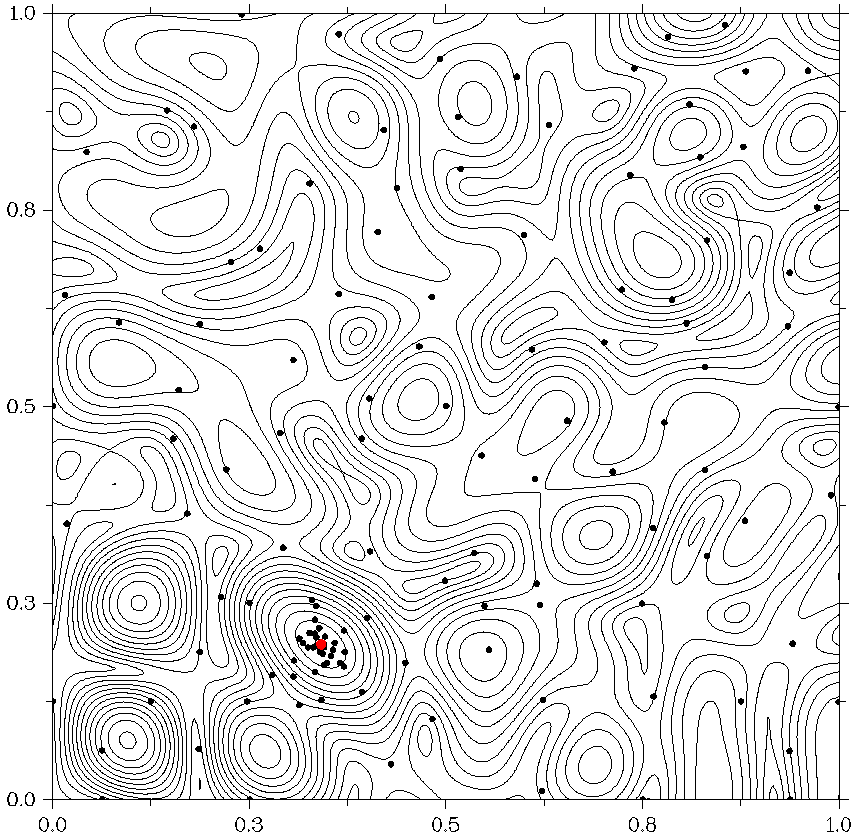
\includegraphics[width=1.0\linewidth]{grishagin.png} \\ (a)}
\end{minipage}
\begin{minipage}{0.48\linewidth}
\center{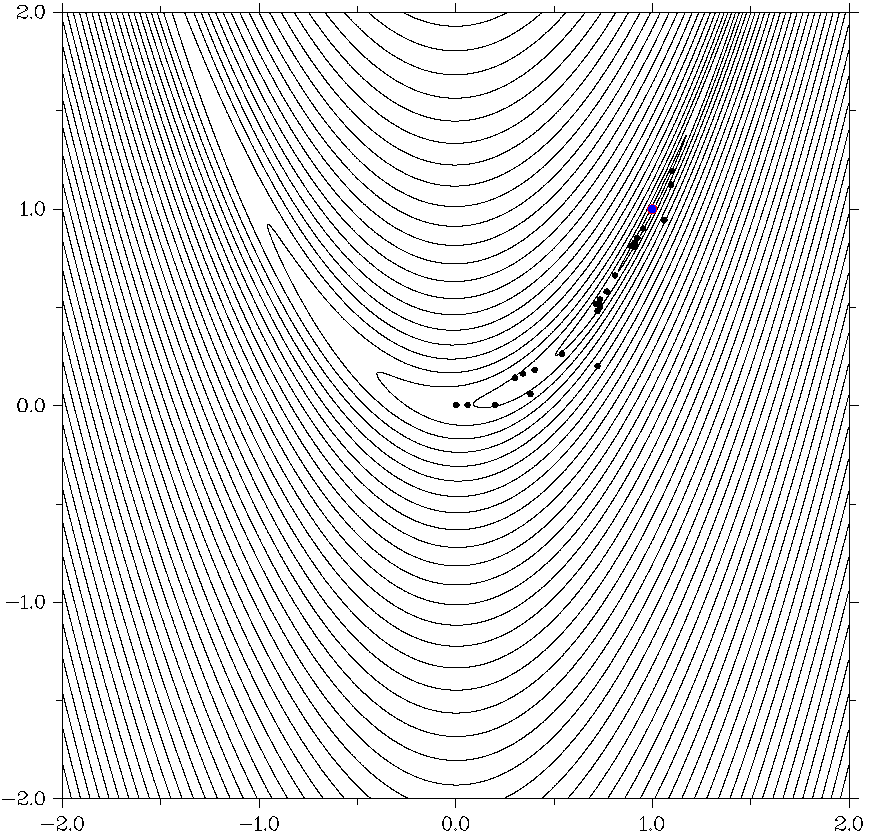
\includegraphics[width=1.0\linewidth]{rosenbrock.png} \\ (b)}
\end{minipage}
\caption{Contour plot of the functions (a) $G(y)$ and (b) $R(x)$}
\label{fig_level}
\end{figure}

In Fig.~\ref{fig_level}, the trial points performed by the global search algorithm and Hooke--Jeeves 
method when solving corresponding problems are marked also. 
The positions of the trial points demonstrate clearly the multiextremality of the function $G(y)$ (the 
trial points form a nonuniform coverage of the search domain) as well as the ravine character 
of the function $R(x)$ (the trial points form an elongated group along the ravine bottom).

The problem was considered to be solved if in the course of minimization of the function $G(y)$, the 
global search algorithm generates the next trial point $y^k$ in the $\epsilon$-nearness of the global 
minimum $y^*$, i.e. $\left\|y^* - y^k\right\|\leq\epsilon$, where $\epsilon = 10^{-2}$. 
At that, the precision of finding the minimum when minimizing the unimodal function $R(x)$ was 
selected 1000 times lower, i.e. $\delta = 10^{-5}$.
In the global search algorithm, the parameter $r=4.5$ from (\ref{Rule_R}) and the evolvent building 
parameter $m=10$ were used; the local Hooke--Jeeves method employed has no additional parameters.

In the first series of experiments, 100 problems of the kind (\ref{test_problem}) were solved, in which 
the dimensionality of the local subproblems was $N=50$. The problems were solved using 1, 4, and 8 
cluster nodes, in which from 2 up to 32 MPI-processes were employed. According to the 
parallelization scheme presented in Fig.~\ref{MPI_tree}, the solving of the global optimization 
problem at the upper nesting level was performed in a single (master) process, which initiated the 
parallel solving of the local problems of the lower level (from 1 up to 31 problems, respectively). So 
far, the minimum possible number of processes employed was equals to 2, one per each nesting level.

Table \ref{tab1} presents the averaged number of iterations $K_{av}$ performed by the global search 
algorithm when minimizing the function $G(y)$, the averaged time of solving the whole problem 
$T_{av}$, and the speed-up in time $S$ subject to the number of employed MPI-processes $p$. 

\begin{table}
\centering
\caption{Results of solving a series of problems of dimensionality $N=52$}\label{tab1}
\begin{tabular}{cccc}
\hline\noalign{\smallskip}
 $\;\;\;p\;\;\;$  &  $\;\;\;K_{av}\;\;\;$ &  $\;\;\;T_{av}\;\;\;$ & $\;\;\;S\;\;\;$ \\
\noalign{\smallskip}\hline\noalign{\smallskip}
 2  & 349.4  & 9.14 & ---  \\
 16 & 25.6   & 0.70 & 13.2 \\
 32 & 12.9   & 0.37 & 24.6 \\
\noalign{\smallskip}\hline
\end{tabular}
\end{table}


In the second series of experiments, 10 problems of the kind (\ref{test_problem}) were solved, in 
which the dimensionality of the local subproblems was equal $N=100$. The running parameters were 
the same as in the previous series of experiments. The results of solving are presented in Table 
\ref{tab2}.

\begin{table}
\centering
\caption{Results of solving a series of problems of dimensionality $N=102$}\label{tab2}
\begin{tabular}{cccc}
\hline\noalign{\smallskip}
 $\;\;\;p\;\;\;$  &  $\;\;\;K_{av}\;\;\;$ &  $\;\;\;T_{av}\;\;\;$ & $\;\;\;S\;\;\;$ \\
\noalign{\smallskip}\hline\noalign{\smallskip}
 2  & 299.1  & 41.19 & ---  \\
 16 & 22.0   & 2.92 & 14.1 \\
 32 & 11.7   & 1.50 & 27.4 \\
\noalign{\smallskip}\hline
\end{tabular}
\end{table}


\section{Conclusion}

The results of experiments performed on the series of the optimization problems
%, in which a multiextremal part and a unimodal one can be selected,
demonstrated the scheme of the 
parallel computations proposed in the present work to have a good potential for parallelization. 
In particular, when solving a series of 100 problems with total number of variables equal to 52 (from 
which, two first variables cause a global effect on the objective function and fifty affected this one 
locally), a speedup of 24.6 has been obtained when using  32 processes. 
In the case of solving  the problems with more complex local subproblems (with the number of the 
local variables $N=100$), the speedup increased up to 27.4 when using 32 processes.
The developed scheme of parallel computations can be applied in the identification of complex 
mathematical models, which are featured by a large number (tens and hundreds) of unknown 
parameters.

%
% ---- Bibliography ----
%
\bibliographystyle{spmpsci}
\bibliography{bibliography}{}

\end{document}
